% ============================================================
% Compact supplementary material for:
% Rethinking Reservoir Pruning: A Dynamical Perspective for
% Echo State Networks
%
% Include after the bibliography:
% % ============================================================
% Compact supplementary material for:
% Rethinking Reservoir Pruning: A Dynamical Perspective for
% Echo State Networks
%
% Include after the bibliography:
% % ============================================================
% Compact supplementary material for:
% Rethinking Reservoir Pruning: A Dynamical Perspective for
% Echo State Networks
%
% Include after the bibliography:
% % ============================================================
% Compact supplementary material for:
% Rethinking Reservoir Pruning: A Dynamical Perspective for
% Echo State Networks
%
% Include after the bibliography:
% \input{supplementary/supplementary}
%
% Required packages in the main preamble:
% \usepackage{booktabs}
% \usepackage{graphicx}
% ============================================================

\clearpage
\appendix

\setcounter{table}{0}
\renewcommand{\thetable}{S\arabic{table}}
\setcounter{figure}{0}
\renewcommand{\thefigure}{S\arabic{figure}}

\section{Additional Experimental Results}
\label{app:additional_results}

This supplement provides an expanded matched-baseline comparison, a compact
paired-seed analysis, two visualizations of the Temperature results, and an
autonomous dynamical evaluation. The main-paper ablation and efficiency table
is not repeated.

% ============================================================
\subsection{Comparison with Additional Pruning Criteria}
\label{app:additional_baselines}

Table~\ref{tab:supp_matched_pruning} extends the controlled comparison to
magnitude, activation-variance, Jacobian column-energy, and betweenness
pruning. The Jacobian baseline ranks neuron $i$ using
\[
s_i^{\mathrm{Jac}}
=
\mathcal{G}_{ii}
=
\frac{1}{T}\sum_{t=1}^{T}
\left\|J_{:,i}(t)\right\|_2^2,
\]
which is the trajectory-averaged squared column norm of the transition
Jacobian. All pruned variants in this table use post-pruning
spectral-radius rescaling. No criterion is uniformly best: DMP+$\rho$
performs best on Temperature, while other methods lead on the remaining
datasets.

\begin{table*}[t]
\centering
\caption{
Matched one-shot reservoir pruning at forecasting horizon $h=20$.
Values are mean $\pm$ standard deviation over ten paired seeds; lower is
better. All pruned variants use post-pruning spectral-radius rescaling.
}
\label{tab:supp_matched_pruning}
\small
\resizebox{\linewidth}{!}{%
\begin{tabular}{lcccccccc}
\toprule
\textbf{Dataset}
& \textbf{Full ESN}
& \textbf{Fresh smaller ESN}
& \textbf{Random+$\rho$}
& \textbf{Magnitude+$\rho$}
& \textbf{Activation variance+$\rho$}
& \textbf{Jacobian col. energy+$\rho$}
& \textbf{Betweenness+$\rho$}
& \textbf{DMP+$\rho$} \\
\midrule
Electricity
& $1.1074 \pm 0.1515$
& $\mathbf{1.0275 \pm 0.0731}$
& $1.0483 \pm 0.1542$
& $1.0349 \pm 0.1436$
& $1.1351 \pm 0.1697$
& $1.0677 \pm 0.1052$
& $1.0882 \pm 0.1609$
& $1.0893 \pm 0.1825$ \\

Mackey--Glass
& $0.4094 \pm 0.0278$
& $0.4132 \pm 0.0107$
& $0.4016 \pm 0.0206$
& $0.4044 \pm 0.0285$
& $\mathbf{0.3778 \pm 0.0252}$
& $0.4172 \pm 0.0165$
& $0.3950 \pm 0.0165$
& $0.4048 \pm 0.0279$ \\

Solar
& $0.8989 \pm 0.0921$
& $0.8591 \pm 0.0477$
& $\mathbf{0.8407 \pm 0.0816}$
& $0.8681 \pm 0.0654$
& $0.9536 \pm 0.0920$
& $0.8575 \pm 0.0649$
& $0.8654 \pm 0.0524$
& $0.8698 \pm 0.0486$ \\

Temperature
& $1.3084 \pm 0.1002$
& $1.2426 \pm 0.1302$
& $1.2485 \pm 0.1419$
& $1.1981 \pm 0.1207$
& $1.7147 \pm 0.5623$
& $1.2080 \pm 0.0923$
& $1.2054 \pm 0.0861$
& $\mathbf{1.1885 \pm 0.1035}$ \\

Wind
& $1.2115 \pm 0.0824$
& $1.2011 \pm 0.1412$
& $1.2394 \pm 0.0806$
& $\mathbf{1.1707 \pm 0.0828}$
& $1.4719 \pm 0.2237$
& $1.1850 \pm 0.0513$
& $1.2544 \pm 0.1398$
& $1.1968 \pm 0.1004$ \\
\bottomrule
\end{tabular}%
}
\end{table*}

% ============================================================
\subsection{Paired-Seed Consistency}
\label{app:paired_consistency}

Table~\ref{tab:paired_consistency} summarizes the ten paired runs without
listing every seed separately. The differences between DMP and random
pruning are generally small and vary across datasets. Spectral rescaling
benefits DMP primarily on Mackey--Glass and is unfavorable on most other
datasets.

\begin{table}[t]
\centering
\caption{
Paired-seed comparison at $N=1000\rightarrow800$ and $h=20$.
$\Delta_{\mathrm{D-R}}$ is DMP NRMSE minus random-pruning NRMSE, and
$\Delta_{\rho}$ is DMP+$\rho$ NRMSE minus DMP NRMSE. Negative values favor
DMP in the first comparison and spectral rescaling in the second. Win counts
are out of ten paired seeds.
}
\label{tab:paired_consistency}
\small
\setlength{\tabcolsep}{4.5pt}
\renewcommand{\arraystretch}{1.12}
\begin{tabular}{lrrrrr}
\toprule
\textbf{Dataset}
& \textbf{Mean $\Delta_{\mathrm{D-R}}$}
& \textbf{Median $\Delta_{\mathrm{D-R}}$}
& \textbf{DMP wins}
& \textbf{Mean $\Delta_{\rho}$}
& \textbf{No-rescale wins} \\
\midrule
Electricity   & $-0.0026$ & $-0.0017$ & $5/10$ & $ 0.2039$ & $10/10$ \\
Mackey--Glass & $-0.0121$ & $-0.0132$ & $9/10$ & $-0.0345$ & $ 1/10$ \\
Solar         & $ 0.0054$ & $ 0.0076$ & $3/10$ & $ 0.1002$ & $10/10$ \\
Temperature   & $-0.0103$ & $ 0.0166$ & $4/10$ & $ 0.0565$ & $ 9/10$ \\
Wind          & $ 0.0114$ & $ 0.0044$ & $3/10$ & $ 0.1193$ & $ 9/10$ \\
\bottomrule
\end{tabular}
\end{table}

% ============================================================
\subsection{Temperature Case Study}
\label{app:temperature_case}

Figure~\ref{fig:supp_temperature_comparison} shows the expanded comparison
on Temperature. DMP+$\rho$ attains the lowest mean NRMSE among the rescaled
methods, although its margin over magnitude, betweenness, and Jacobian
column-energy pruning is small.

% The figure uses the same Jacobian column-energy terminology as Table~\ref{tab:supp_matched_pruning}.
\begin{figure*}[t]
\centering
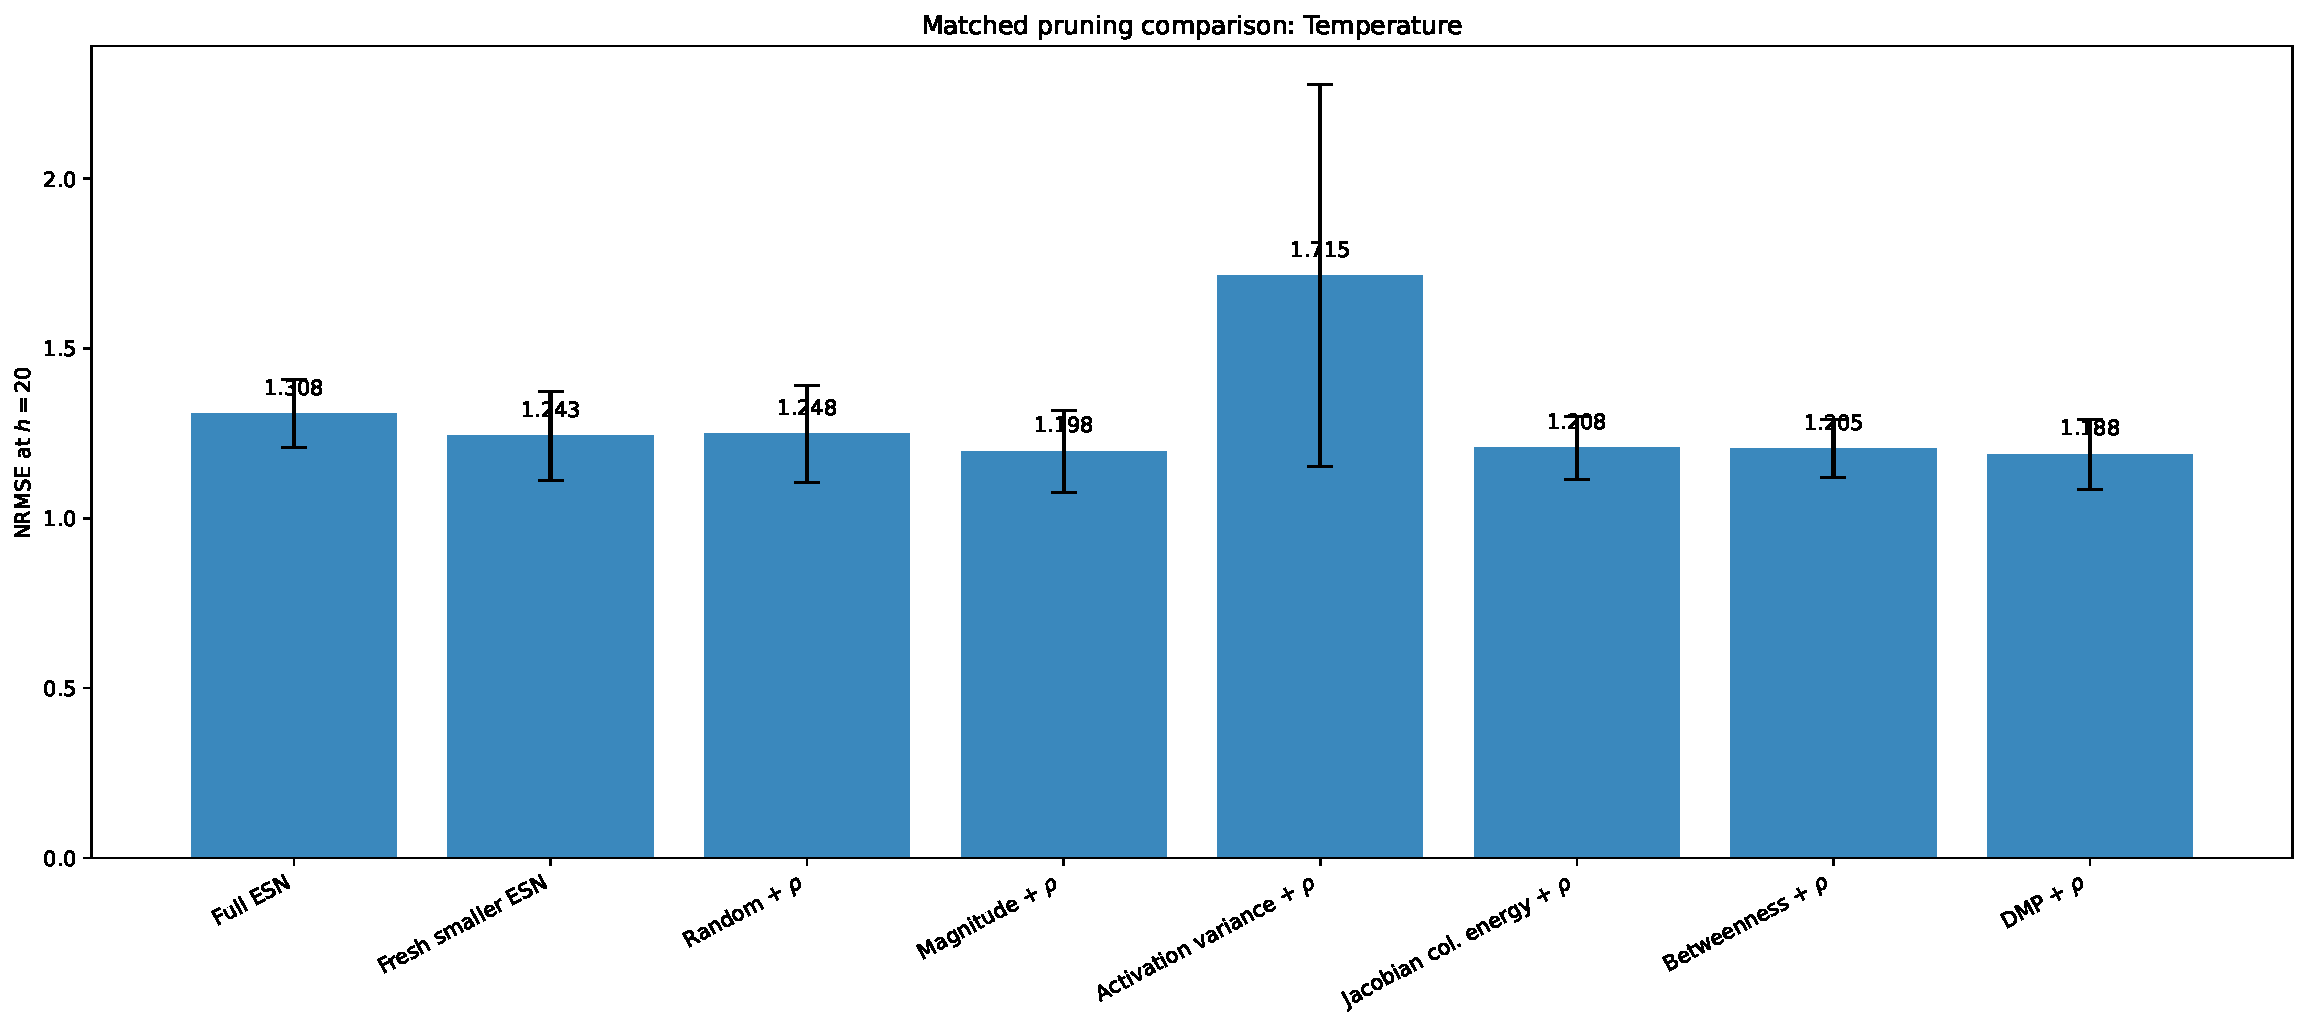
\includegraphics[width=0.90\textwidth]
{figures/temperature_matched_pruning_nrmse.pdf}
\caption{
Matched pruning comparison on Temperature at $h=20$ over ten paired seeds.
Bars show mean NRMSE, and error bars show one standard deviation. All pruned
variants shown in this figure use post-pruning spectral-radius rescaling.
}
\label{fig:supp_temperature_comparison}
\end{figure*}

Figure~\ref{fig:supp_temperature_tradeoff} relates forecasting error to
inference latency. The reduced reservoirs occupy a similar low-latency
range, while DMP without rescaling gives the lowest mean NRMSE on this
dataset.

\begin{figure*}[t]
\centering
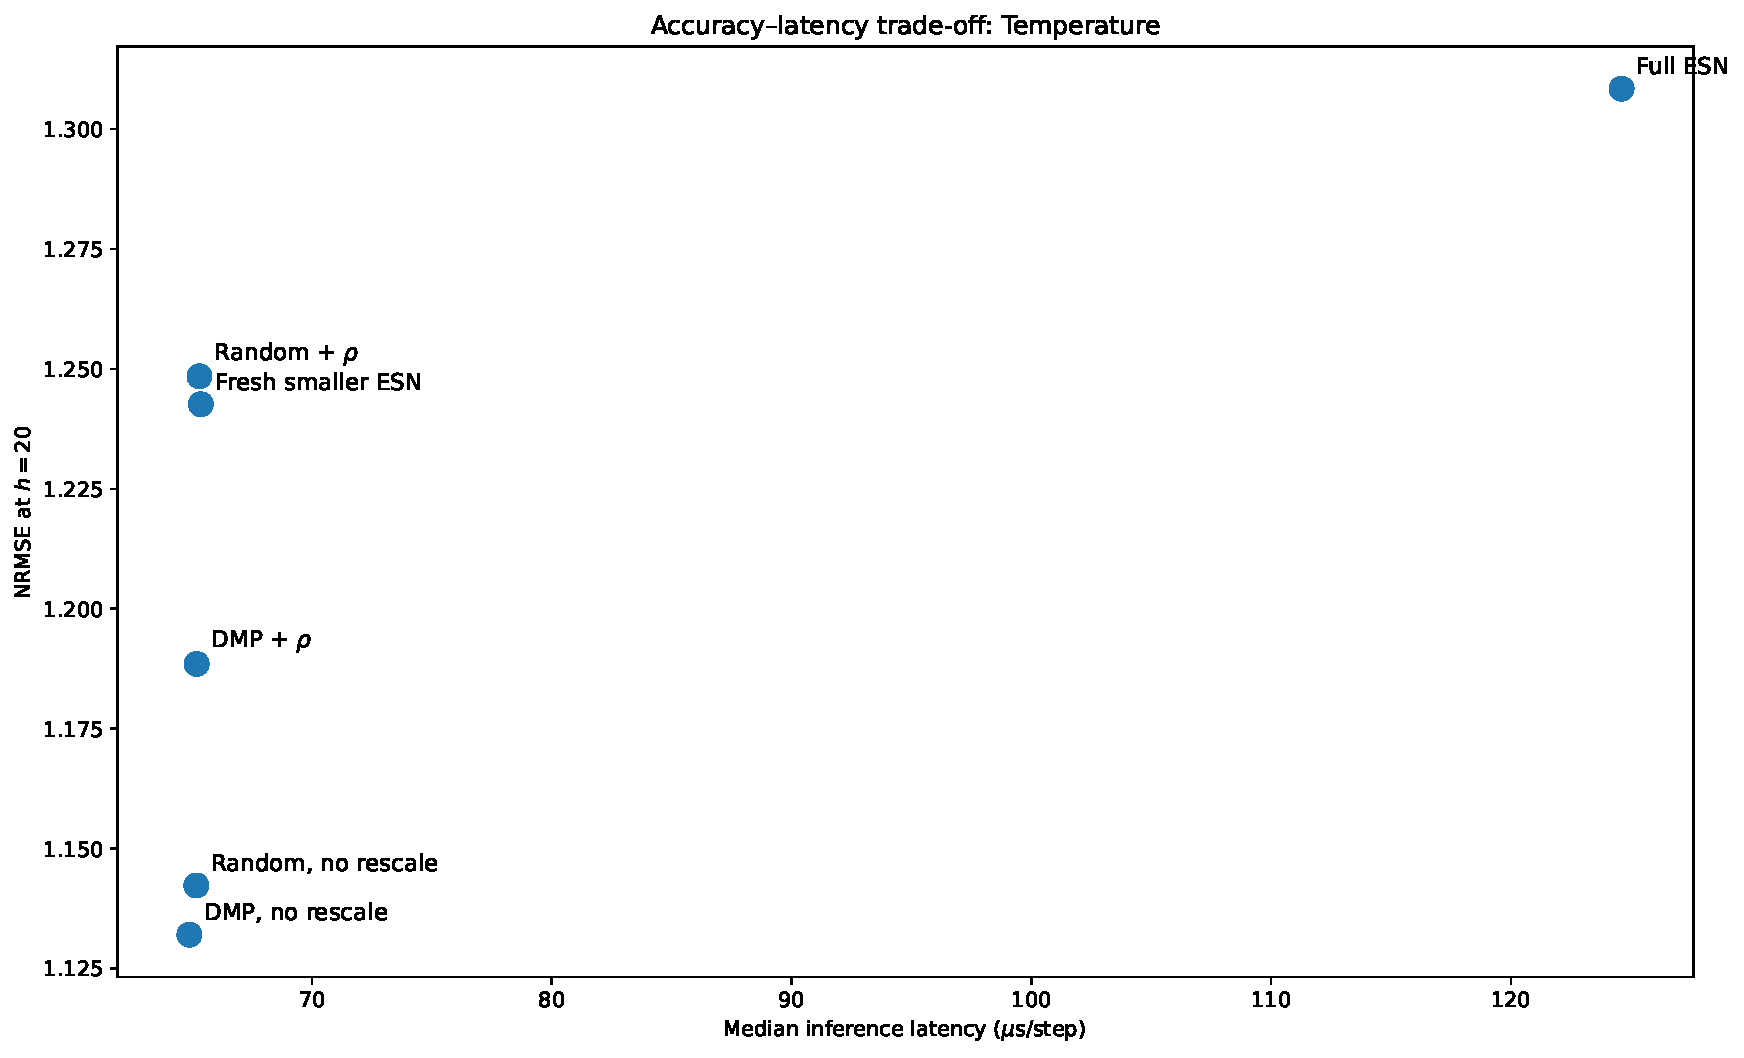
\includegraphics[width=0.90\textwidth]
{figures/temperature_accuracy_latency.pdf}
\caption{
Accuracy--latency comparison on Temperature after reducing the reservoir
from $N=1000$ to $N=800$. Lower values on both axes are preferred.
}
\label{fig:supp_temperature_tradeoff}
\end{figure*}

% ============================================================
\subsection{Autonomous Dynamical Evaluation}
\label{app:dynamical_fidelity}

The autonomous evaluation uses a one-step readout in closed loop, with each
prediction fed back as the next input. The valid prediction length is the
number of steps before the absolute error first exceeds $0.40$ target
standard deviations, and the valid fraction is this length divided by the
total rollout length. Power spectral density (PSD) distance is the
total-variation distance between the normalized target and predicted power
spectra. Autocorrelation-function (ACF) distance is the root mean squared
difference between their autocorrelation sequences up to lag 100.

Table~\ref{tab:dynamical_fidelity} shows that all methods have similarly
short valid prediction windows on Mackey--Glass. DMP+$\rho$ does not
consistently improve rollout NRMSE, PSD distance, or ACF distance, indicating
that improved driven forecasting does not necessarily imply closer
autonomous chaotic statistics.

\begin{table*}[t]
\centering
\caption{
Autonomous dynamical-fidelity evaluation on Mackey--Glass. Values are
mean $\pm$ standard deviation over ten seeds. Lower is better, except for
valid steps and valid fraction.
}
\label{tab:dynamical_fidelity}
\small
\setlength{\tabcolsep}{5pt}
\renewcommand{\arraystretch}{1.12}
\begin{tabular}{lccccc}
\toprule
\textbf{Method}
& \textbf{Rollout NRMSE}
& \textbf{Valid steps $\uparrow$}
& \textbf{Valid fraction $\uparrow$}
& \textbf{PSD distance}
& \textbf{ACF distance} \\
\midrule
Full ESN
& $0.4538 \pm 0.0195$
& $8.0 \pm 0.0$
& $0.080 \pm 0.000$
& $\mathbf{0.1962 \pm 0.0164}$
& $\mathbf{0.0493 \pm 0.0136}$ \\

Fresh $N=800$ ESN
& $0.4499 \pm 0.0272$
& $8.0 \pm 0.0$
& $0.080 \pm 0.000$
& $0.2016 \pm 0.0177$
& $0.0535 \pm 0.0105$ \\

Random+$\rho$
& $\mathbf{0.4443 \pm 0.0250}$
& $8.0 \pm 0.0$
& $0.080 \pm 0.000$
& $0.1964 \pm 0.0203$
& $0.0512 \pm 0.0138$ \\

DMP+$\rho$
& $0.4615 \pm 0.0307$
& $\mathbf{8.1 \pm 0.3}$
& $\mathbf{0.081 \pm 0.003}$
& $0.2070 \pm 0.0139$
& $0.0573 \pm 0.0090$ \\
\bottomrule
\end{tabular}
\end{table*}

%
% Required packages in the main preamble:
% \usepackage{booktabs}
% \usepackage{graphicx}
% ============================================================

\clearpage
\appendix

\setcounter{table}{0}
\renewcommand{\thetable}{S\arabic{table}}
\setcounter{figure}{0}
\renewcommand{\thefigure}{S\arabic{figure}}

\section{Additional Experimental Results}
\label{app:additional_results}

This supplement provides an expanded matched-baseline comparison, a compact
paired-seed analysis, two visualizations of the Temperature results, and an
autonomous dynamical evaluation. The main-paper ablation and efficiency table
is not repeated.

% ============================================================
\subsection{Comparison with Additional Pruning Criteria}
\label{app:additional_baselines}

Table~\ref{tab:supp_matched_pruning} extends the controlled comparison to
magnitude, activation-variance, Jacobian column-energy, and betweenness
pruning. The Jacobian baseline ranks neuron $i$ using
\[
s_i^{\mathrm{Jac}}
=
\mathcal{G}_{ii}
=
\frac{1}{T}\sum_{t=1}^{T}
\left\|J_{:,i}(t)\right\|_2^2,
\]
which is the trajectory-averaged squared column norm of the transition
Jacobian. All pruned variants in this table use post-pruning
spectral-radius rescaling. No criterion is uniformly best: DMP+$\rho$
performs best on Temperature, while other methods lead on the remaining
datasets.

\begin{table*}[t]
\centering
\caption{
Matched one-shot reservoir pruning at forecasting horizon $h=20$.
Values are mean $\pm$ standard deviation over ten paired seeds; lower is
better. All pruned variants use post-pruning spectral-radius rescaling.
}
\label{tab:supp_matched_pruning}
\small
\resizebox{\linewidth}{!}{%
\begin{tabular}{lcccccccc}
\toprule
\textbf{Dataset}
& \textbf{Full ESN}
& \textbf{Fresh smaller ESN}
& \textbf{Random+$\rho$}
& \textbf{Magnitude+$\rho$}
& \textbf{Activation variance+$\rho$}
& \textbf{Jacobian col. energy+$\rho$}
& \textbf{Betweenness+$\rho$}
& \textbf{DMP+$\rho$} \\
\midrule
Electricity
& $1.1074 \pm 0.1515$
& $\mathbf{1.0275 \pm 0.0731}$
& $1.0483 \pm 0.1542$
& $1.0349 \pm 0.1436$
& $1.1351 \pm 0.1697$
& $1.0677 \pm 0.1052$
& $1.0882 \pm 0.1609$
& $1.0893 \pm 0.1825$ \\

Mackey--Glass
& $0.4094 \pm 0.0278$
& $0.4132 \pm 0.0107$
& $0.4016 \pm 0.0206$
& $0.4044 \pm 0.0285$
& $\mathbf{0.3778 \pm 0.0252}$
& $0.4172 \pm 0.0165$
& $0.3950 \pm 0.0165$
& $0.4048 \pm 0.0279$ \\

Solar
& $0.8989 \pm 0.0921$
& $0.8591 \pm 0.0477$
& $\mathbf{0.8407 \pm 0.0816}$
& $0.8681 \pm 0.0654$
& $0.9536 \pm 0.0920$
& $0.8575 \pm 0.0649$
& $0.8654 \pm 0.0524$
& $0.8698 \pm 0.0486$ \\

Temperature
& $1.3084 \pm 0.1002$
& $1.2426 \pm 0.1302$
& $1.2485 \pm 0.1419$
& $1.1981 \pm 0.1207$
& $1.7147 \pm 0.5623$
& $1.2080 \pm 0.0923$
& $1.2054 \pm 0.0861$
& $\mathbf{1.1885 \pm 0.1035}$ \\

Wind
& $1.2115 \pm 0.0824$
& $1.2011 \pm 0.1412$
& $1.2394 \pm 0.0806$
& $\mathbf{1.1707 \pm 0.0828}$
& $1.4719 \pm 0.2237$
& $1.1850 \pm 0.0513$
& $1.2544 \pm 0.1398$
& $1.1968 \pm 0.1004$ \\
\bottomrule
\end{tabular}%
}
\end{table*}

% ============================================================
\subsection{Paired-Seed Consistency}
\label{app:paired_consistency}

Table~\ref{tab:paired_consistency} summarizes the ten paired runs without
listing every seed separately. The differences between DMP and random
pruning are generally small and vary across datasets. Spectral rescaling
benefits DMP primarily on Mackey--Glass and is unfavorable on most other
datasets.

\begin{table}[t]
\centering
\caption{
Paired-seed comparison at $N=1000\rightarrow800$ and $h=20$.
$\Delta_{\mathrm{D-R}}$ is DMP NRMSE minus random-pruning NRMSE, and
$\Delta_{\rho}$ is DMP+$\rho$ NRMSE minus DMP NRMSE. Negative values favor
DMP in the first comparison and spectral rescaling in the second. Win counts
are out of ten paired seeds.
}
\label{tab:paired_consistency}
\small
\setlength{\tabcolsep}{4.5pt}
\renewcommand{\arraystretch}{1.12}
\begin{tabular}{lrrrrr}
\toprule
\textbf{Dataset}
& \textbf{Mean $\Delta_{\mathrm{D-R}}$}
& \textbf{Median $\Delta_{\mathrm{D-R}}$}
& \textbf{DMP wins}
& \textbf{Mean $\Delta_{\rho}$}
& \textbf{No-rescale wins} \\
\midrule
Electricity   & $-0.0026$ & $-0.0017$ & $5/10$ & $ 0.2039$ & $10/10$ \\
Mackey--Glass & $-0.0121$ & $-0.0132$ & $9/10$ & $-0.0345$ & $ 1/10$ \\
Solar         & $ 0.0054$ & $ 0.0076$ & $3/10$ & $ 0.1002$ & $10/10$ \\
Temperature   & $-0.0103$ & $ 0.0166$ & $4/10$ & $ 0.0565$ & $ 9/10$ \\
Wind          & $ 0.0114$ & $ 0.0044$ & $3/10$ & $ 0.1193$ & $ 9/10$ \\
\bottomrule
\end{tabular}
\end{table}

% ============================================================
\subsection{Temperature Case Study}
\label{app:temperature_case}

Figure~\ref{fig:supp_temperature_comparison} shows the expanded comparison
on Temperature. DMP+$\rho$ attains the lowest mean NRMSE among the rescaled
methods, although its margin over magnitude, betweenness, and Jacobian
column-energy pruning is small.

% The figure uses the same Jacobian column-energy terminology as Table~\ref{tab:supp_matched_pruning}.
\begin{figure*}[t]
\centering
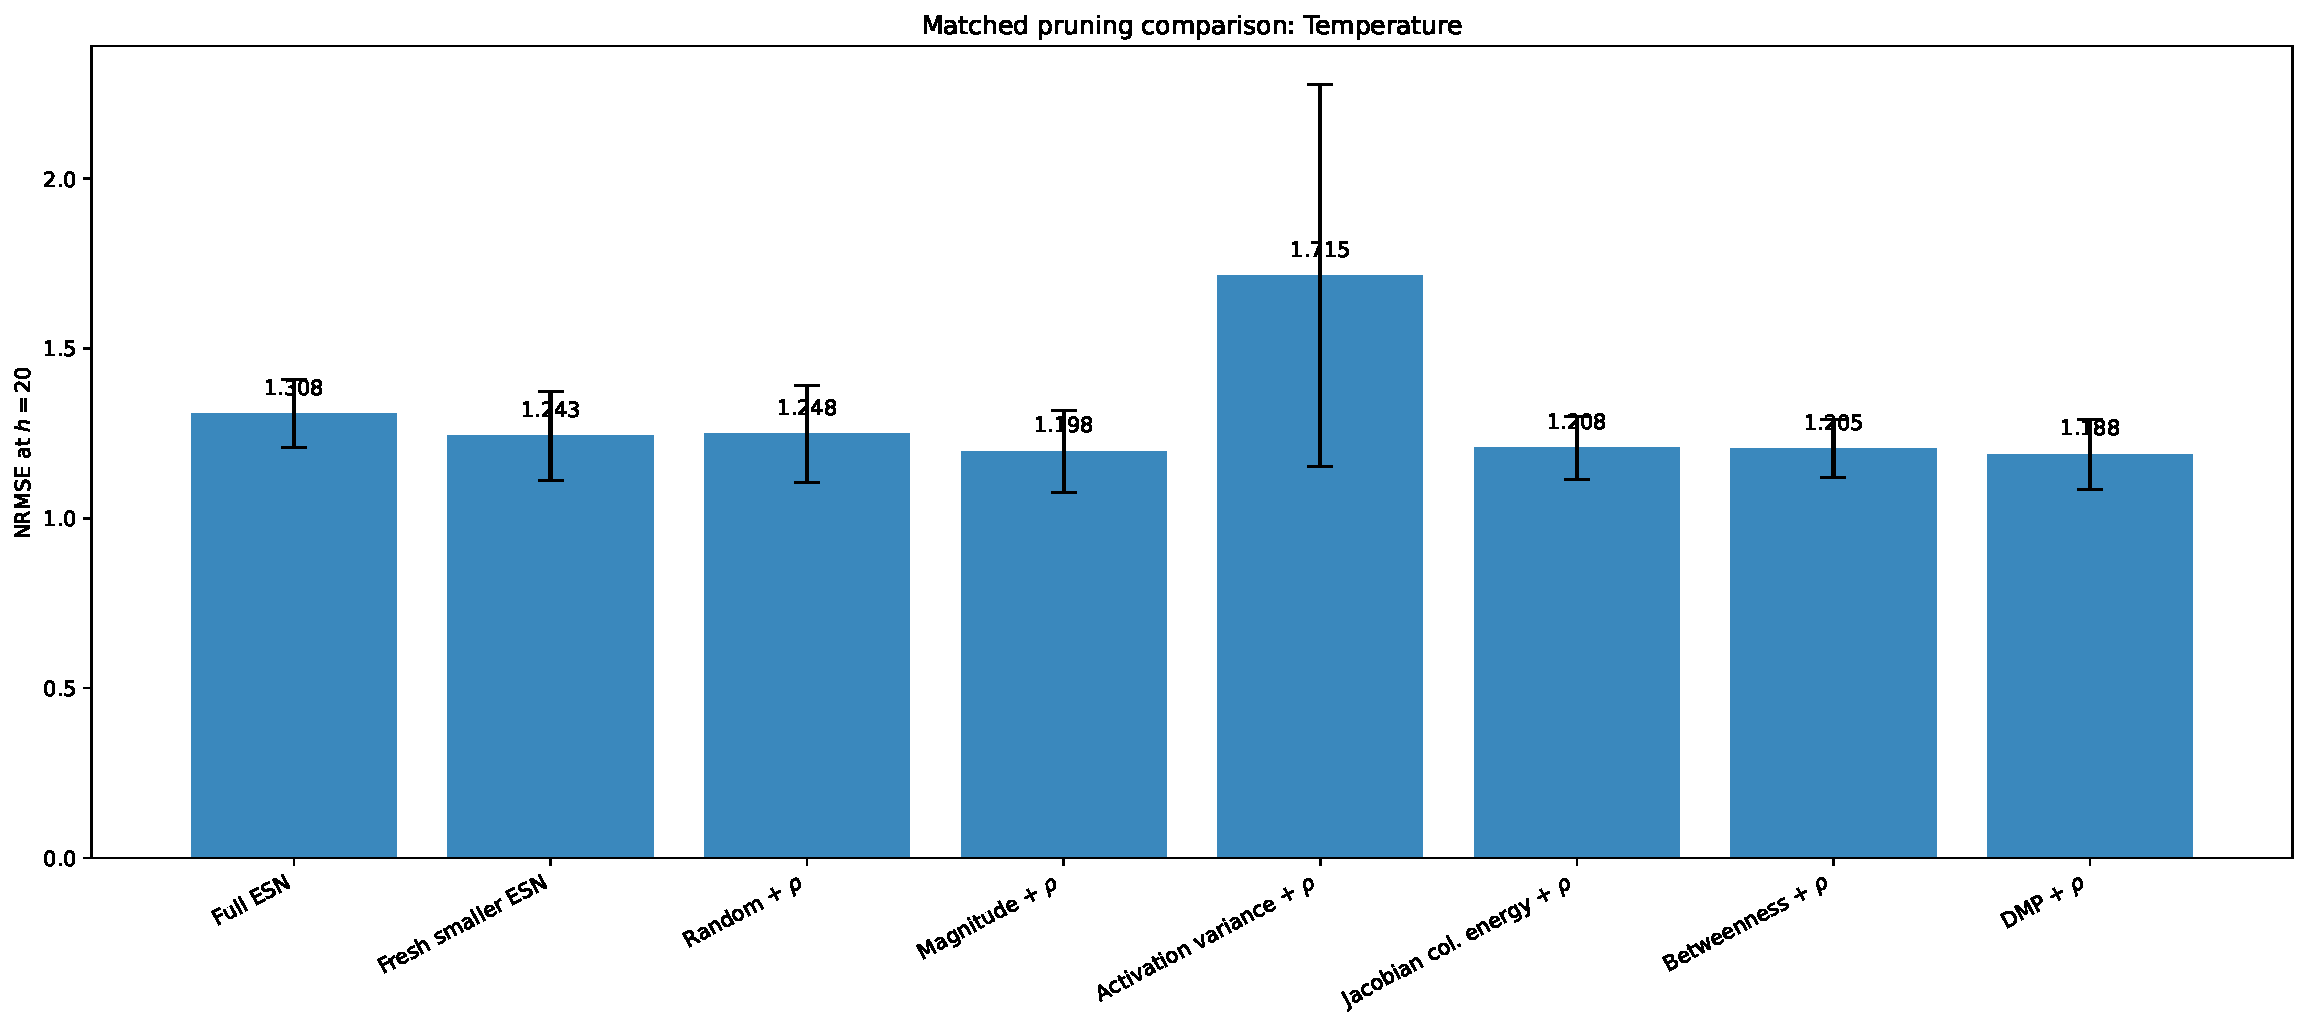
\includegraphics[width=0.90\textwidth]
{figures/temperature_matched_pruning_nrmse.pdf}
\caption{
Matched pruning comparison on Temperature at $h=20$ over ten paired seeds.
Bars show mean NRMSE, and error bars show one standard deviation. All pruned
variants shown in this figure use post-pruning spectral-radius rescaling.
}
\label{fig:supp_temperature_comparison}
\end{figure*}

Figure~\ref{fig:supp_temperature_tradeoff} relates forecasting error to
inference latency. The reduced reservoirs occupy a similar low-latency
range, while DMP without rescaling gives the lowest mean NRMSE on this
dataset.

\begin{figure*}[t]
\centering
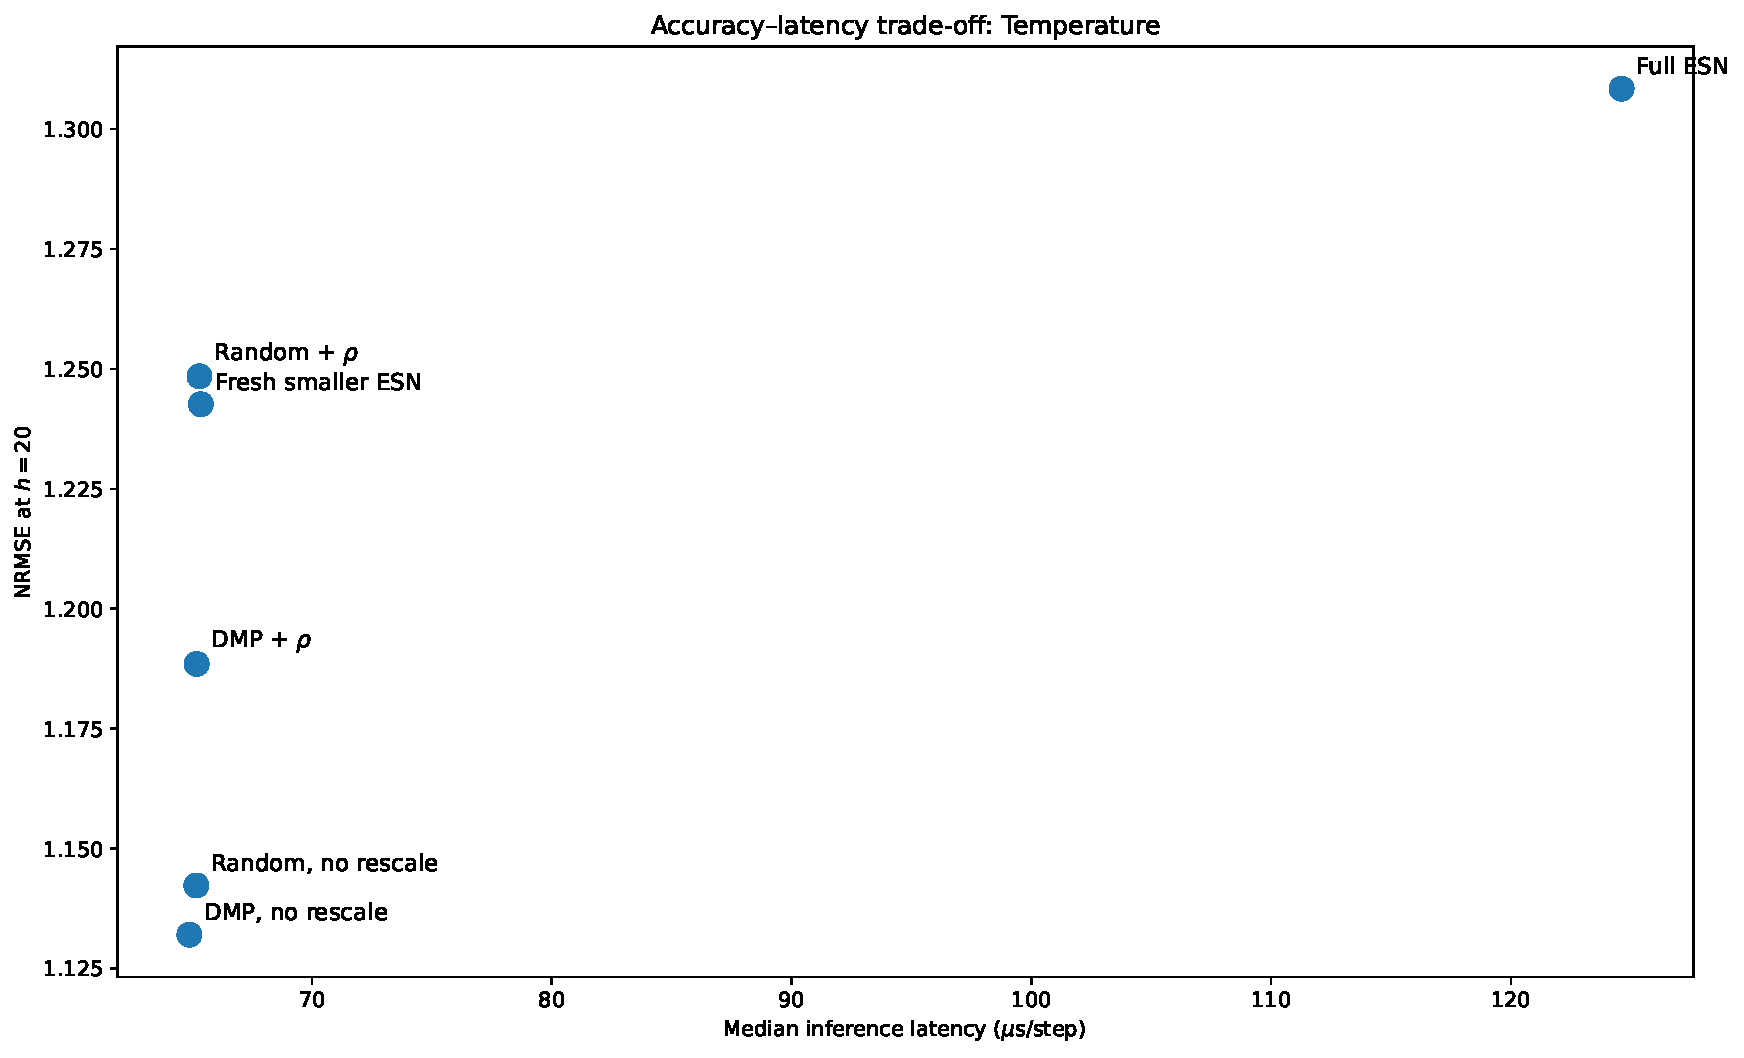
\includegraphics[width=0.90\textwidth]
{figures/temperature_accuracy_latency.pdf}
\caption{
Accuracy--latency comparison on Temperature after reducing the reservoir
from $N=1000$ to $N=800$. Lower values on both axes are preferred.
}
\label{fig:supp_temperature_tradeoff}
\end{figure*}

% ============================================================
\subsection{Autonomous Dynamical Evaluation}
\label{app:dynamical_fidelity}

The autonomous evaluation uses a one-step readout in closed loop, with each
prediction fed back as the next input. The valid prediction length is the
number of steps before the absolute error first exceeds $0.40$ target
standard deviations, and the valid fraction is this length divided by the
total rollout length. Power spectral density (PSD) distance is the
total-variation distance between the normalized target and predicted power
spectra. Autocorrelation-function (ACF) distance is the root mean squared
difference between their autocorrelation sequences up to lag 100.

Table~\ref{tab:dynamical_fidelity} shows that all methods have similarly
short valid prediction windows on Mackey--Glass. DMP+$\rho$ does not
consistently improve rollout NRMSE, PSD distance, or ACF distance, indicating
that improved driven forecasting does not necessarily imply closer
autonomous chaotic statistics.

\begin{table*}[t]
\centering
\caption{
Autonomous dynamical-fidelity evaluation on Mackey--Glass. Values are
mean $\pm$ standard deviation over ten seeds. Lower is better, except for
valid steps and valid fraction.
}
\label{tab:dynamical_fidelity}
\small
\setlength{\tabcolsep}{5pt}
\renewcommand{\arraystretch}{1.12}
\begin{tabular}{lccccc}
\toprule
\textbf{Method}
& \textbf{Rollout NRMSE}
& \textbf{Valid steps $\uparrow$}
& \textbf{Valid fraction $\uparrow$}
& \textbf{PSD distance}
& \textbf{ACF distance} \\
\midrule
Full ESN
& $0.4538 \pm 0.0195$
& $8.0 \pm 0.0$
& $0.080 \pm 0.000$
& $\mathbf{0.1962 \pm 0.0164}$
& $\mathbf{0.0493 \pm 0.0136}$ \\

Fresh $N=800$ ESN
& $0.4499 \pm 0.0272$
& $8.0 \pm 0.0$
& $0.080 \pm 0.000$
& $0.2016 \pm 0.0177$
& $0.0535 \pm 0.0105$ \\

Random+$\rho$
& $\mathbf{0.4443 \pm 0.0250}$
& $8.0 \pm 0.0$
& $0.080 \pm 0.000$
& $0.1964 \pm 0.0203$
& $0.0512 \pm 0.0138$ \\

DMP+$\rho$
& $0.4615 \pm 0.0307$
& $\mathbf{8.1 \pm 0.3}$
& $\mathbf{0.081 \pm 0.003}$
& $0.2070 \pm 0.0139$
& $0.0573 \pm 0.0090$ \\
\bottomrule
\end{tabular}
\end{table*}

%
% Required packages in the main preamble:
% \usepackage{booktabs}
% \usepackage{graphicx}
% ============================================================

\clearpage
\appendix

\setcounter{table}{0}
\renewcommand{\thetable}{S\arabic{table}}
\setcounter{figure}{0}
\renewcommand{\thefigure}{S\arabic{figure}}

\section{Additional Experimental Results}
\label{app:additional_results}

This supplement provides an expanded matched-baseline comparison, a compact
paired-seed analysis, two visualizations of the Temperature results, and an
autonomous dynamical evaluation. The main-paper ablation and efficiency table
is not repeated.

% ============================================================
\subsection{Comparison with Additional Pruning Criteria}
\label{app:additional_baselines}

Table~\ref{tab:supp_matched_pruning} extends the controlled comparison to
magnitude, activation-variance, Jacobian column-energy, and betweenness
pruning. The Jacobian baseline ranks neuron $i$ using
\[
s_i^{\mathrm{Jac}}
=
\mathcal{G}_{ii}
=
\frac{1}{T}\sum_{t=1}^{T}
\left\|J_{:,i}(t)\right\|_2^2,
\]
which is the trajectory-averaged squared column norm of the transition
Jacobian. All pruned variants in this table use post-pruning
spectral-radius rescaling. No criterion is uniformly best: DMP+$\rho$
performs best on Temperature, while other methods lead on the remaining
datasets.

\begin{table*}[t]
\centering
\caption{
Matched one-shot reservoir pruning at forecasting horizon $h=20$.
Values are mean $\pm$ standard deviation over ten paired seeds; lower is
better. All pruned variants use post-pruning spectral-radius rescaling.
}
\label{tab:supp_matched_pruning}
\small
\resizebox{\linewidth}{!}{%
\begin{tabular}{lcccccccc}
\toprule
\textbf{Dataset}
& \textbf{Full ESN}
& \textbf{Fresh smaller ESN}
& \textbf{Random+$\rho$}
& \textbf{Magnitude+$\rho$}
& \textbf{Activation variance+$\rho$}
& \textbf{Jacobian col. energy+$\rho$}
& \textbf{Betweenness+$\rho$}
& \textbf{DMP+$\rho$} \\
\midrule
Electricity
& $1.1074 \pm 0.1515$
& $\mathbf{1.0275 \pm 0.0731}$
& $1.0483 \pm 0.1542$
& $1.0349 \pm 0.1436$
& $1.1351 \pm 0.1697$
& $1.0677 \pm 0.1052$
& $1.0882 \pm 0.1609$
& $1.0893 \pm 0.1825$ \\

Mackey--Glass
& $0.4094 \pm 0.0278$
& $0.4132 \pm 0.0107$
& $0.4016 \pm 0.0206$
& $0.4044 \pm 0.0285$
& $\mathbf{0.3778 \pm 0.0252}$
& $0.4172 \pm 0.0165$
& $0.3950 \pm 0.0165$
& $0.4048 \pm 0.0279$ \\

Solar
& $0.8989 \pm 0.0921$
& $0.8591 \pm 0.0477$
& $\mathbf{0.8407 \pm 0.0816}$
& $0.8681 \pm 0.0654$
& $0.9536 \pm 0.0920$
& $0.8575 \pm 0.0649$
& $0.8654 \pm 0.0524$
& $0.8698 \pm 0.0486$ \\

Temperature
& $1.3084 \pm 0.1002$
& $1.2426 \pm 0.1302$
& $1.2485 \pm 0.1419$
& $1.1981 \pm 0.1207$
& $1.7147 \pm 0.5623$
& $1.2080 \pm 0.0923$
& $1.2054 \pm 0.0861$
& $\mathbf{1.1885 \pm 0.1035}$ \\

Wind
& $1.2115 \pm 0.0824$
& $1.2011 \pm 0.1412$
& $1.2394 \pm 0.0806$
& $\mathbf{1.1707 \pm 0.0828}$
& $1.4719 \pm 0.2237$
& $1.1850 \pm 0.0513$
& $1.2544 \pm 0.1398$
& $1.1968 \pm 0.1004$ \\
\bottomrule
\end{tabular}%
}
\end{table*}

% ============================================================
\subsection{Paired-Seed Consistency}
\label{app:paired_consistency}

Table~\ref{tab:paired_consistency} summarizes the ten paired runs without
listing every seed separately. The differences between DMP and random
pruning are generally small and vary across datasets. Spectral rescaling
benefits DMP primarily on Mackey--Glass and is unfavorable on most other
datasets.

\begin{table}[t]
\centering
\caption{
Paired-seed comparison at $N=1000\rightarrow800$ and $h=20$.
$\Delta_{\mathrm{D-R}}$ is DMP NRMSE minus random-pruning NRMSE, and
$\Delta_{\rho}$ is DMP+$\rho$ NRMSE minus DMP NRMSE. Negative values favor
DMP in the first comparison and spectral rescaling in the second. Win counts
are out of ten paired seeds.
}
\label{tab:paired_consistency}
\small
\setlength{\tabcolsep}{4.5pt}
\renewcommand{\arraystretch}{1.12}
\begin{tabular}{lrrrrr}
\toprule
\textbf{Dataset}
& \textbf{Mean $\Delta_{\mathrm{D-R}}$}
& \textbf{Median $\Delta_{\mathrm{D-R}}$}
& \textbf{DMP wins}
& \textbf{Mean $\Delta_{\rho}$}
& \textbf{No-rescale wins} \\
\midrule
Electricity   & $-0.0026$ & $-0.0017$ & $5/10$ & $ 0.2039$ & $10/10$ \\
Mackey--Glass & $-0.0121$ & $-0.0132$ & $9/10$ & $-0.0345$ & $ 1/10$ \\
Solar         & $ 0.0054$ & $ 0.0076$ & $3/10$ & $ 0.1002$ & $10/10$ \\
Temperature   & $-0.0103$ & $ 0.0166$ & $4/10$ & $ 0.0565$ & $ 9/10$ \\
Wind          & $ 0.0114$ & $ 0.0044$ & $3/10$ & $ 0.1193$ & $ 9/10$ \\
\bottomrule
\end{tabular}
\end{table}

% ============================================================
\subsection{Temperature Case Study}
\label{app:temperature_case}

Figure~\ref{fig:supp_temperature_comparison} shows the expanded comparison
on Temperature. DMP+$\rho$ attains the lowest mean NRMSE among the rescaled
methods, although its margin over magnitude, betweenness, and Jacobian
column-energy pruning is small.

% The figure uses the same Jacobian column-energy terminology as Table~\ref{tab:supp_matched_pruning}.
\begin{figure*}[t]
\centering
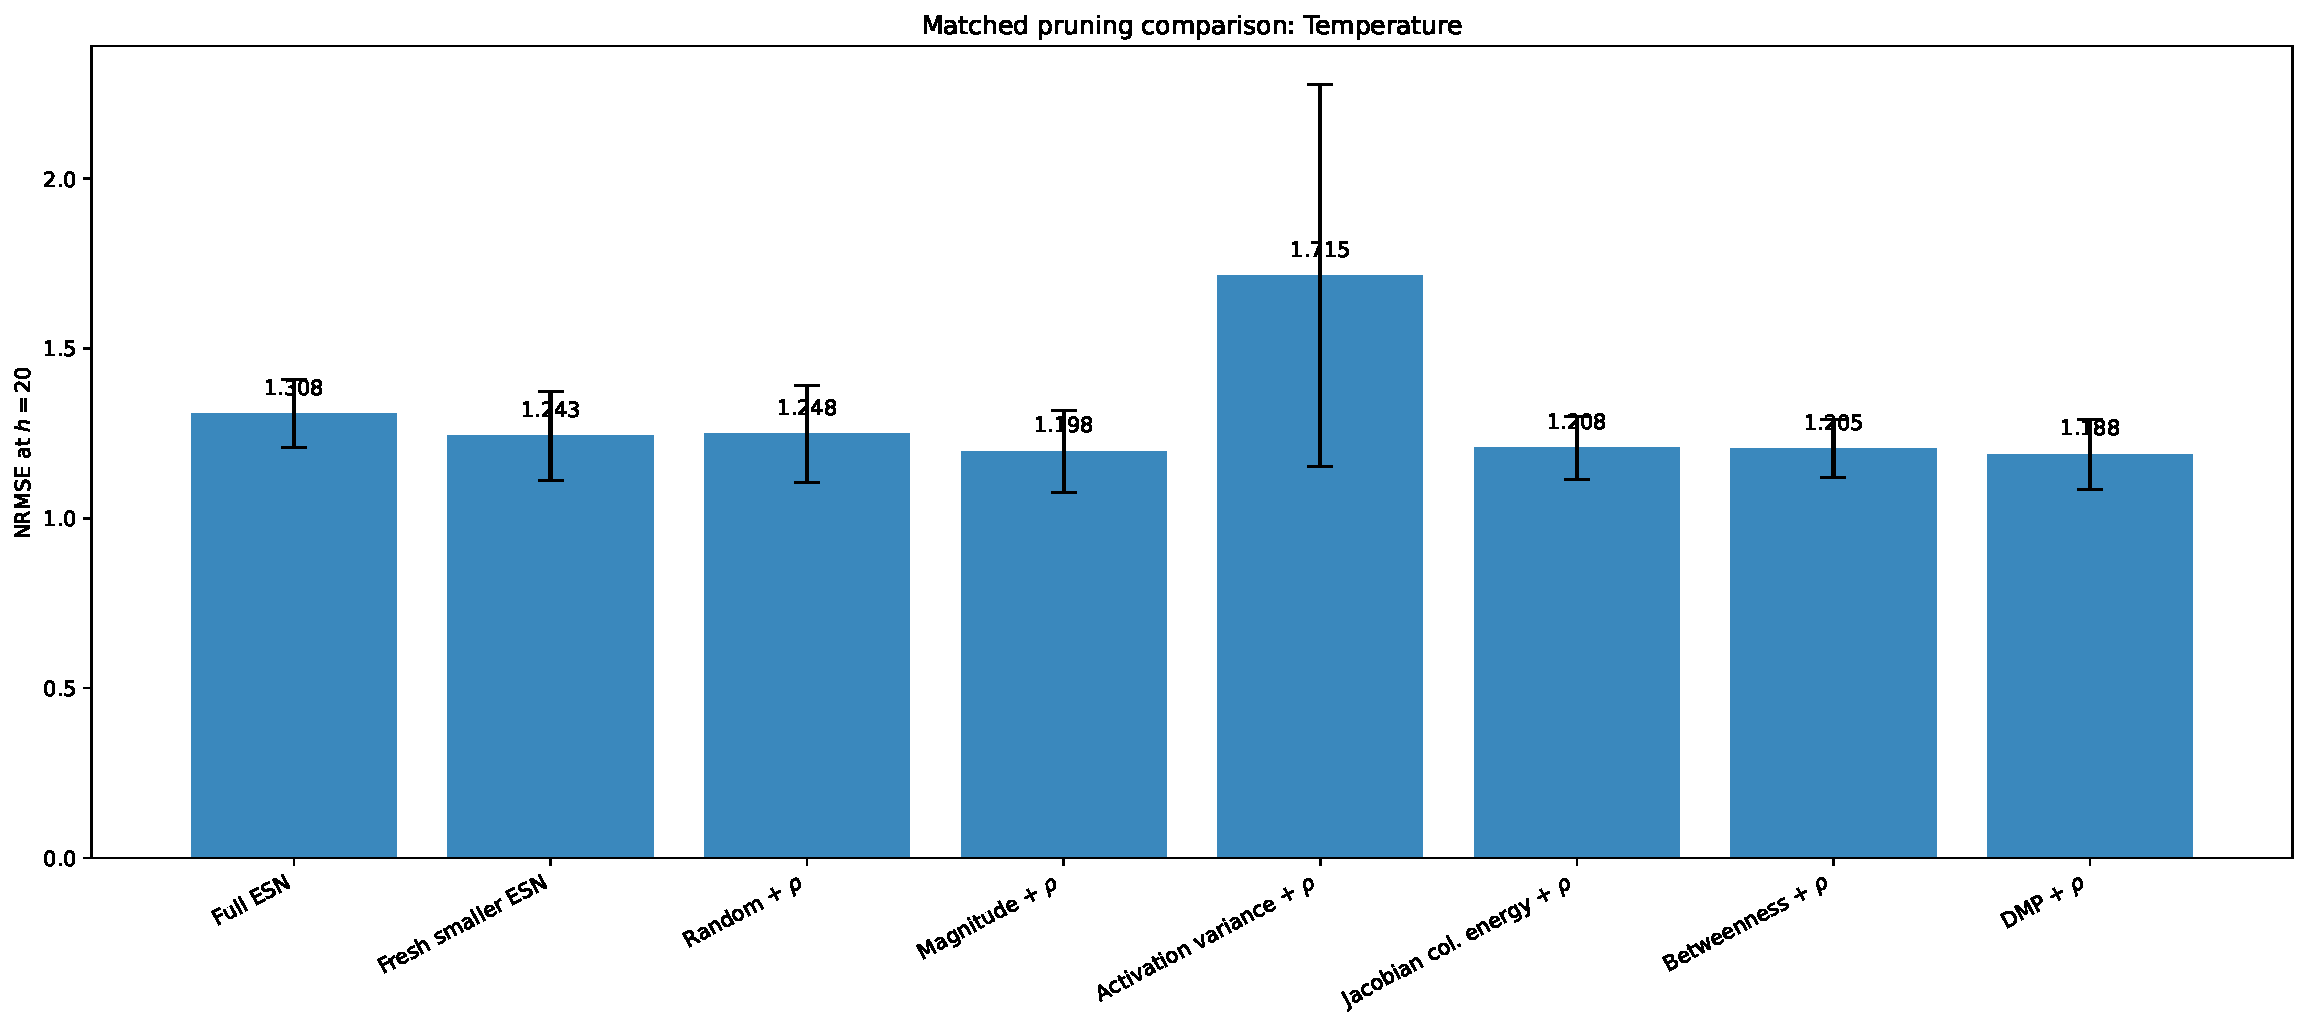
\includegraphics[width=0.90\textwidth]
{figures/temperature_matched_pruning_nrmse.pdf}
\caption{
Matched pruning comparison on Temperature at $h=20$ over ten paired seeds.
Bars show mean NRMSE, and error bars show one standard deviation. All pruned
variants shown in this figure use post-pruning spectral-radius rescaling.
}
\label{fig:supp_temperature_comparison}
\end{figure*}

Figure~\ref{fig:supp_temperature_tradeoff} relates forecasting error to
inference latency. The reduced reservoirs occupy a similar low-latency
range, while DMP without rescaling gives the lowest mean NRMSE on this
dataset.

\begin{figure*}[t]
\centering
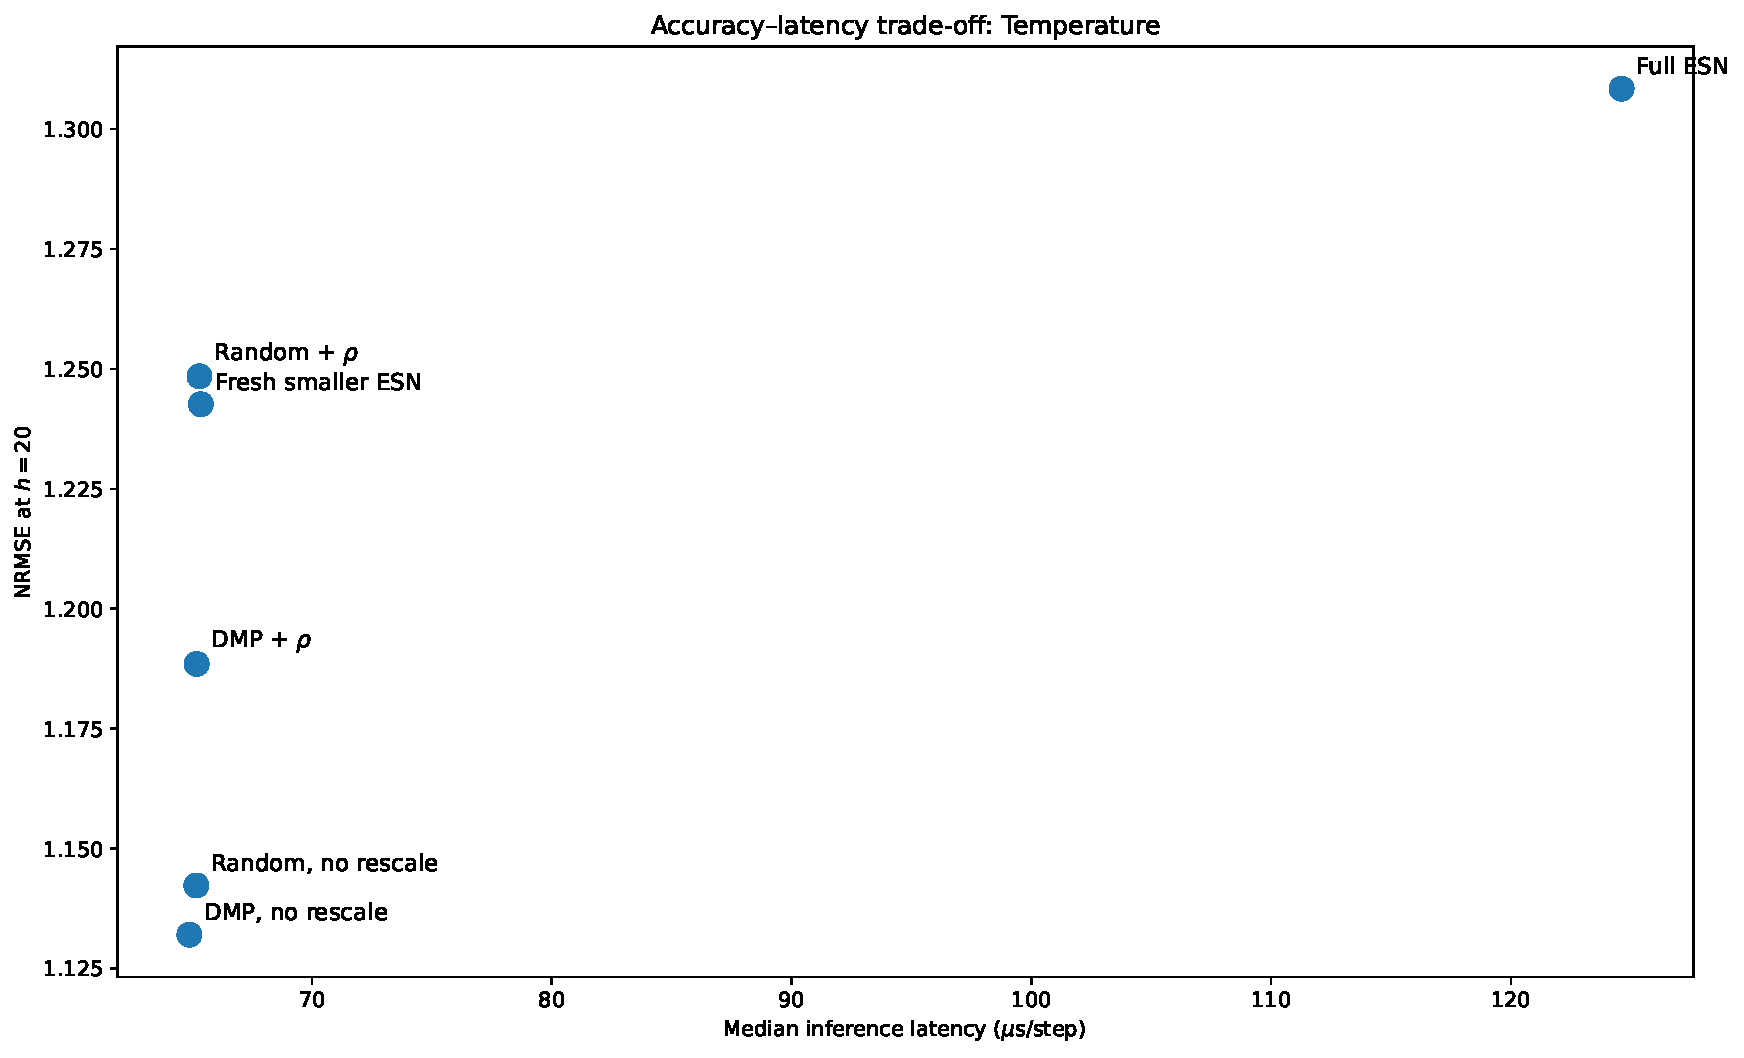
\includegraphics[width=0.90\textwidth]
{figures/temperature_accuracy_latency.pdf}
\caption{
Accuracy--latency comparison on Temperature after reducing the reservoir
from $N=1000$ to $N=800$. Lower values on both axes are preferred.
}
\label{fig:supp_temperature_tradeoff}
\end{figure*}

% ============================================================
\subsection{Autonomous Dynamical Evaluation}
\label{app:dynamical_fidelity}

The autonomous evaluation uses a one-step readout in closed loop, with each
prediction fed back as the next input. The valid prediction length is the
number of steps before the absolute error first exceeds $0.40$ target
standard deviations, and the valid fraction is this length divided by the
total rollout length. Power spectral density (PSD) distance is the
total-variation distance between the normalized target and predicted power
spectra. Autocorrelation-function (ACF) distance is the root mean squared
difference between their autocorrelation sequences up to lag 100.

Table~\ref{tab:dynamical_fidelity} shows that all methods have similarly
short valid prediction windows on Mackey--Glass. DMP+$\rho$ does not
consistently improve rollout NRMSE, PSD distance, or ACF distance, indicating
that improved driven forecasting does not necessarily imply closer
autonomous chaotic statistics.

\begin{table*}[t]
\centering
\caption{
Autonomous dynamical-fidelity evaluation on Mackey--Glass. Values are
mean $\pm$ standard deviation over ten seeds. Lower is better, except for
valid steps and valid fraction.
}
\label{tab:dynamical_fidelity}
\small
\setlength{\tabcolsep}{5pt}
\renewcommand{\arraystretch}{1.12}
\begin{tabular}{lccccc}
\toprule
\textbf{Method}
& \textbf{Rollout NRMSE}
& \textbf{Valid steps $\uparrow$}
& \textbf{Valid fraction $\uparrow$}
& \textbf{PSD distance}
& \textbf{ACF distance} \\
\midrule
Full ESN
& $0.4538 \pm 0.0195$
& $8.0 \pm 0.0$
& $0.080 \pm 0.000$
& $\mathbf{0.1962 \pm 0.0164}$
& $\mathbf{0.0493 \pm 0.0136}$ \\

Fresh $N=800$ ESN
& $0.4499 \pm 0.0272$
& $8.0 \pm 0.0$
& $0.080 \pm 0.000$
& $0.2016 \pm 0.0177$
& $0.0535 \pm 0.0105$ \\

Random+$\rho$
& $\mathbf{0.4443 \pm 0.0250}$
& $8.0 \pm 0.0$
& $0.080 \pm 0.000$
& $0.1964 \pm 0.0203$
& $0.0512 \pm 0.0138$ \\

DMP+$\rho$
& $0.4615 \pm 0.0307$
& $\mathbf{8.1 \pm 0.3}$
& $\mathbf{0.081 \pm 0.003}$
& $0.2070 \pm 0.0139$
& $0.0573 \pm 0.0090$ \\
\bottomrule
\end{tabular}
\end{table*}

%
% Required packages in the main preamble:
% \usepackage{booktabs}
% \usepackage{graphicx}
% ============================================================

\clearpage
\appendix

\setcounter{table}{0}
\renewcommand{\thetable}{S\arabic{table}}
\setcounter{figure}{0}
\renewcommand{\thefigure}{S\arabic{figure}}

\section{Additional Experimental Results}
\label{app:additional_results}

This supplement provides an expanded matched-baseline comparison, a compact
paired-seed analysis, two visualizations of the Temperature results, and an
autonomous dynamical evaluation. The main-paper ablation and efficiency table
is not repeated.

% ============================================================
\subsection{Comparison with Additional Pruning Criteria}
\label{app:additional_baselines}

Table~\ref{tab:supp_matched_pruning} extends the controlled comparison to
magnitude, activation-variance, Jacobian column-energy, and betweenness
pruning. The Jacobian baseline ranks neuron $i$ using
\[
s_i^{\mathrm{Jac}}
=
\mathcal{G}_{ii}
=
\frac{1}{T}\sum_{t=1}^{T}
\left\|J_{:,i}(t)\right\|_2^2,
\]
which is the trajectory-averaged squared column norm of the transition
Jacobian. All pruned variants in this table use post-pruning
spectral-radius rescaling. No criterion is uniformly best: DMP+$\rho$
performs best on Temperature, while other methods lead on the remaining
datasets.

\begin{table*}[t]
\centering
\caption{
Matched one-shot reservoir pruning at forecasting horizon $h=20$.
Values are mean $\pm$ standard deviation over ten paired seeds; lower is
better. All pruned variants use post-pruning spectral-radius rescaling.
}
\label{tab:supp_matched_pruning}
\small
\resizebox{\linewidth}{!}{%
\begin{tabular}{lcccccccc}
\toprule
\textbf{Dataset}
& \textbf{Full ESN}
& \textbf{Fresh smaller ESN}
& \textbf{Random+$\rho$}
& \textbf{Magnitude+$\rho$}
& \textbf{Activation variance+$\rho$}
& \textbf{Jacobian col. energy+$\rho$}
& \textbf{Betweenness+$\rho$}
& \textbf{DMP+$\rho$} \\
\midrule
Electricity
& $1.1074 \pm 0.1515$
& $\mathbf{1.0275 \pm 0.0731}$
& $1.0483 \pm 0.1542$
& $1.0349 \pm 0.1436$
& $1.1351 \pm 0.1697$
& $1.0677 \pm 0.1052$
& $1.0882 \pm 0.1609$
& $1.0893 \pm 0.1825$ \\

Mackey--Glass
& $0.4094 \pm 0.0278$
& $0.4132 \pm 0.0107$
& $0.4016 \pm 0.0206$
& $0.4044 \pm 0.0285$
& $\mathbf{0.3778 \pm 0.0252}$
& $0.4172 \pm 0.0165$
& $0.3950 \pm 0.0165$
& $0.4048 \pm 0.0279$ \\

Solar
& $0.8989 \pm 0.0921$
& $0.8591 \pm 0.0477$
& $\mathbf{0.8407 \pm 0.0816}$
& $0.8681 \pm 0.0654$
& $0.9536 \pm 0.0920$
& $0.8575 \pm 0.0649$
& $0.8654 \pm 0.0524$
& $0.8698 \pm 0.0486$ \\

Temperature
& $1.3084 \pm 0.1002$
& $1.2426 \pm 0.1302$
& $1.2485 \pm 0.1419$
& $1.1981 \pm 0.1207$
& $1.7147 \pm 0.5623$
& $1.2080 \pm 0.0923$
& $1.2054 \pm 0.0861$
& $\mathbf{1.1885 \pm 0.1035}$ \\

Wind
& $1.2115 \pm 0.0824$
& $1.2011 \pm 0.1412$
& $1.2394 \pm 0.0806$
& $\mathbf{1.1707 \pm 0.0828}$
& $1.4719 \pm 0.2237$
& $1.1850 \pm 0.0513$
& $1.2544 \pm 0.1398$
& $1.1968 \pm 0.1004$ \\
\bottomrule
\end{tabular}%
}
\end{table*}

% ============================================================
\subsection{Paired-Seed Consistency}
\label{app:paired_consistency}

Table~\ref{tab:paired_consistency} summarizes the ten paired runs without
listing every seed separately. The differences between DMP and random
pruning are generally small and vary across datasets. Spectral rescaling
benefits DMP primarily on Mackey--Glass and is unfavorable on most other
datasets.

\begin{table}[t]
\centering
\caption{
Paired-seed comparison at $N=1000\rightarrow800$ and $h=20$.
$\Delta_{\mathrm{D-R}}$ is DMP NRMSE minus random-pruning NRMSE, and
$\Delta_{\rho}$ is DMP+$\rho$ NRMSE minus DMP NRMSE. Negative values favor
DMP in the first comparison and spectral rescaling in the second. Win counts
are out of ten paired seeds.
}
\label{tab:paired_consistency}
\small
\setlength{\tabcolsep}{4.5pt}
\renewcommand{\arraystretch}{1.12}
\begin{tabular}{lrrrrr}
\toprule
\textbf{Dataset}
& \textbf{Mean $\Delta_{\mathrm{D-R}}$}
& \textbf{Median $\Delta_{\mathrm{D-R}}$}
& \textbf{DMP wins}
& \textbf{Mean $\Delta_{\rho}$}
& \textbf{No-rescale wins} \\
\midrule
Electricity   & $-0.0026$ & $-0.0017$ & $5/10$ & $ 0.2039$ & $10/10$ \\
Mackey--Glass & $-0.0121$ & $-0.0132$ & $9/10$ & $-0.0345$ & $ 1/10$ \\
Solar         & $ 0.0054$ & $ 0.0076$ & $3/10$ & $ 0.1002$ & $10/10$ \\
Temperature   & $-0.0103$ & $ 0.0166$ & $4/10$ & $ 0.0565$ & $ 9/10$ \\
Wind          & $ 0.0114$ & $ 0.0044$ & $3/10$ & $ 0.1193$ & $ 9/10$ \\
\bottomrule
\end{tabular}
\end{table}

% ============================================================
\subsection{Temperature Case Study}
\label{app:temperature_case}

Figure~\ref{fig:supp_temperature_comparison} shows the expanded comparison
on Temperature. DMP+$\rho$ attains the lowest mean NRMSE among the rescaled
methods, although its margin over magnitude, betweenness, and Jacobian
column-energy pruning is small.

% The figure uses the same Jacobian column-energy terminology as Table~\ref{tab:supp_matched_pruning}.
\begin{figure*}[t]
\centering
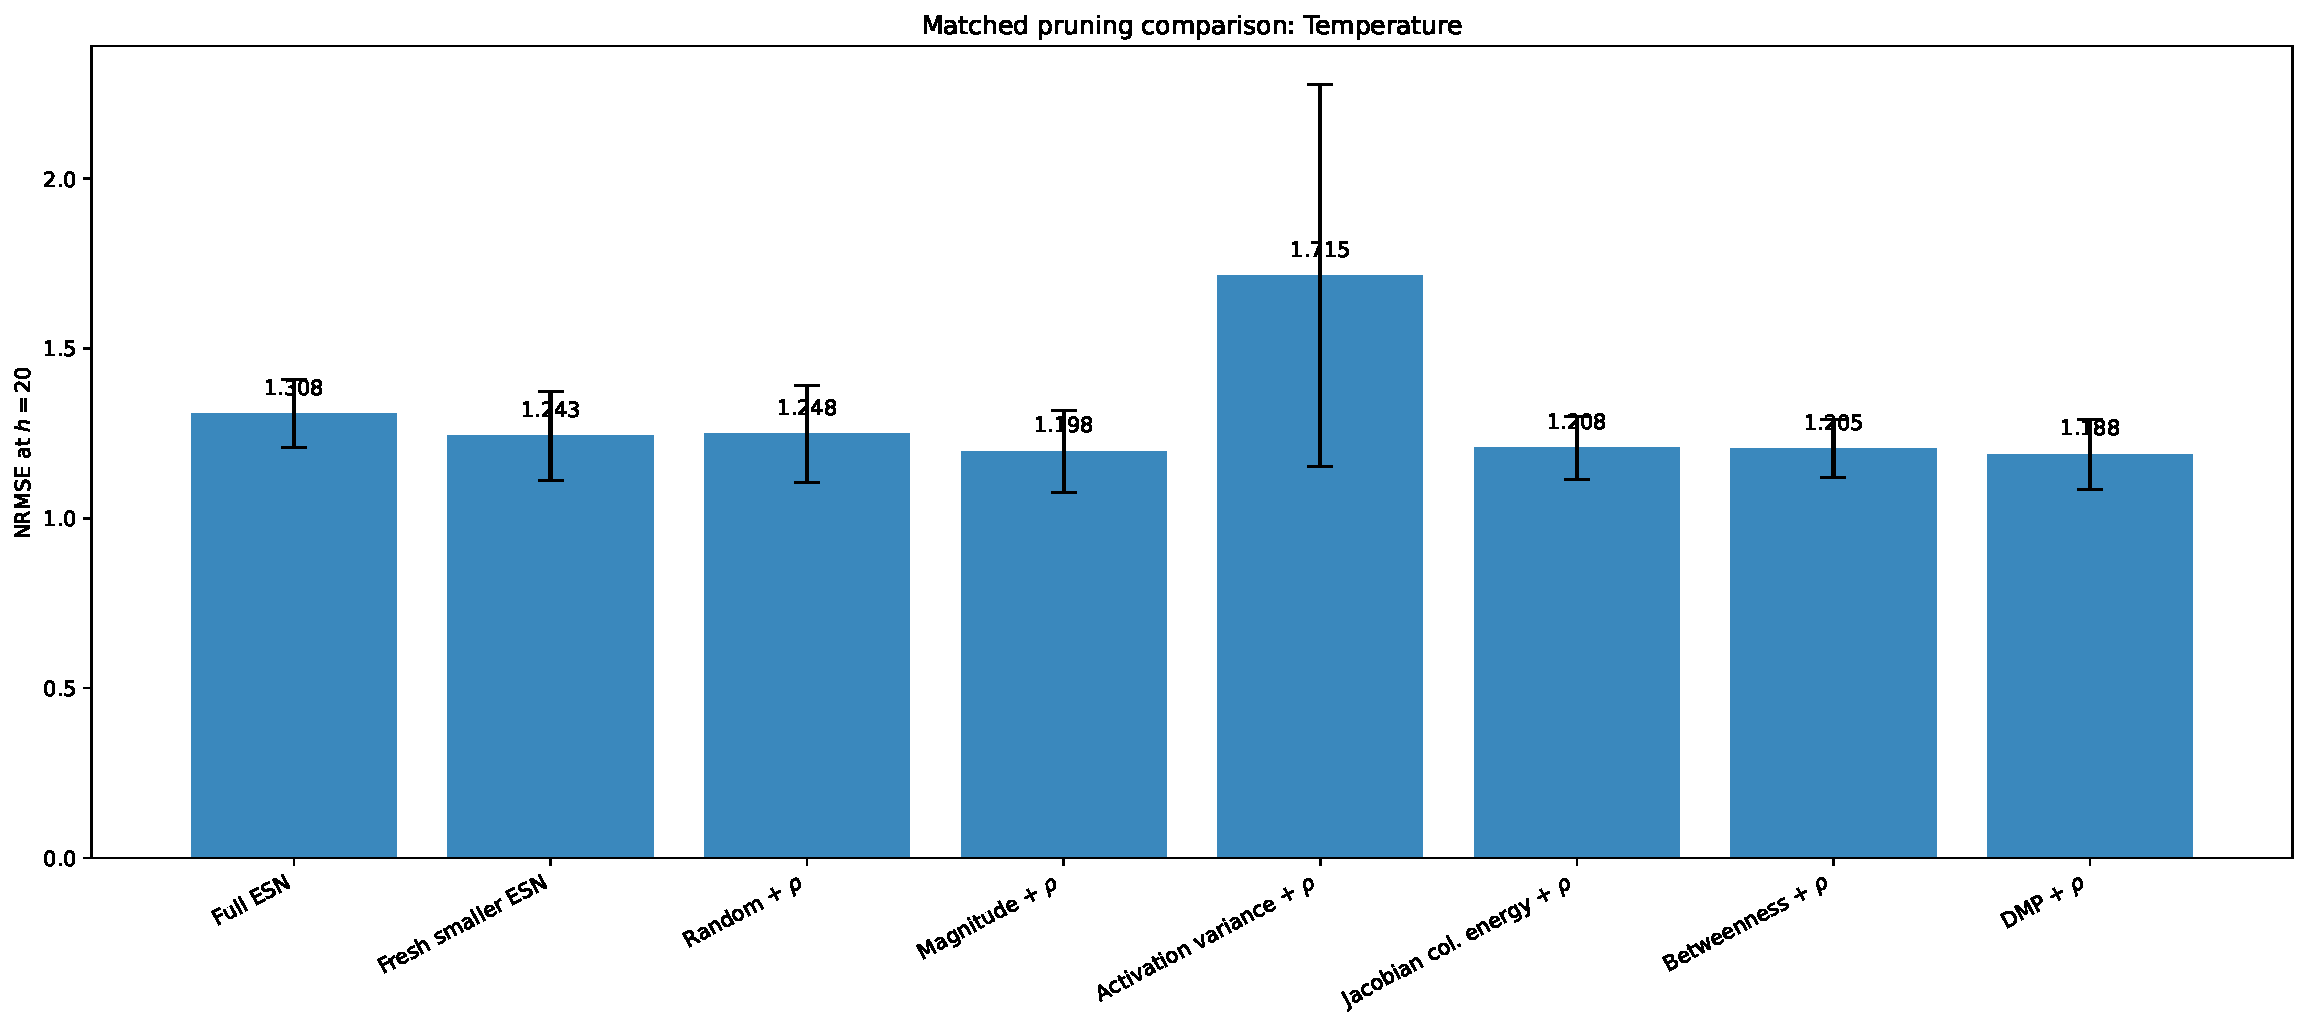
\includegraphics[width=0.90\textwidth]
{figures/temperature_matched_pruning_nrmse.pdf}
\caption{
Matched pruning comparison on Temperature at $h=20$ over ten paired seeds.
Bars show mean NRMSE, and error bars show one standard deviation. All pruned
variants shown in this figure use post-pruning spectral-radius rescaling.
}
\label{fig:supp_temperature_comparison}
\end{figure*}

Figure~\ref{fig:supp_temperature_tradeoff} relates forecasting error to
inference latency. The reduced reservoirs occupy a similar low-latency
range, while DMP without rescaling gives the lowest mean NRMSE on this
dataset.

\begin{figure*}[t]
\centering
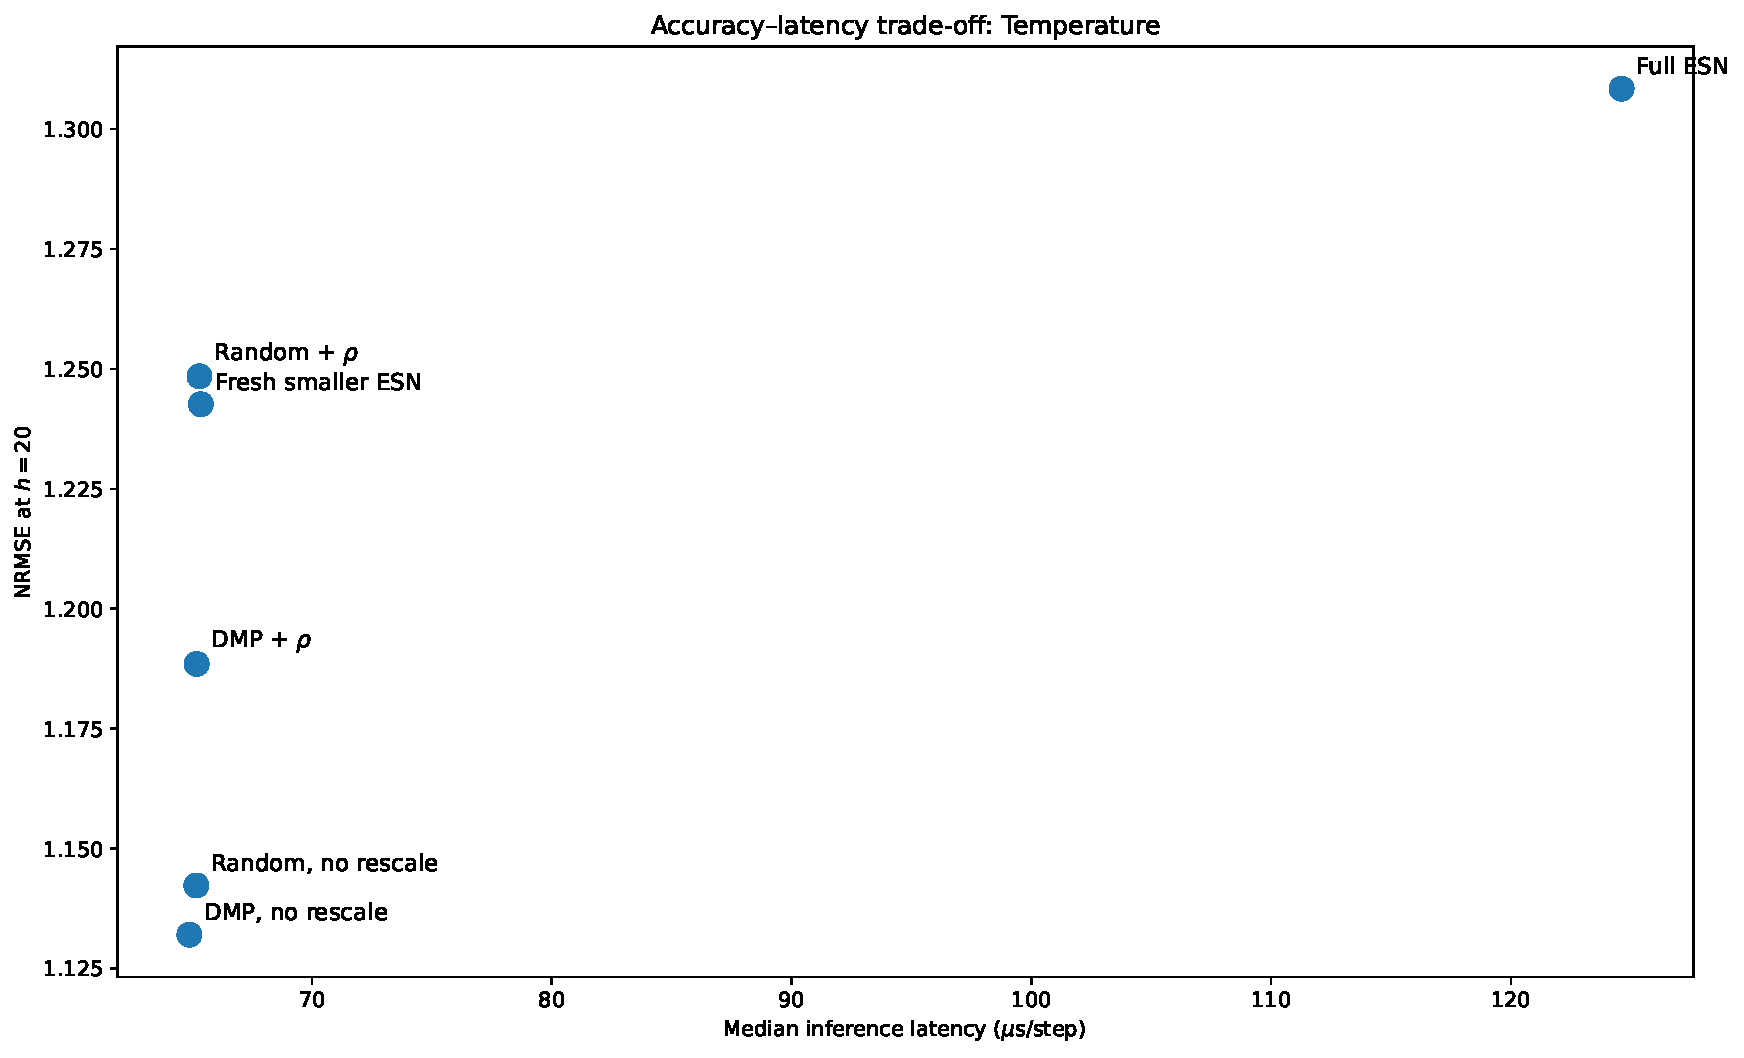
\includegraphics[width=0.90\textwidth]
{figures/temperature_accuracy_latency.pdf}
\caption{
Accuracy--latency comparison on Temperature after reducing the reservoir
from $N=1000$ to $N=800$. Lower values on both axes are preferred.
}
\label{fig:supp_temperature_tradeoff}
\end{figure*}

% ============================================================
\subsection{Autonomous Dynamical Evaluation}
\label{app:dynamical_fidelity}

The autonomous evaluation uses a one-step readout in closed loop, with each
prediction fed back as the next input. The valid prediction length is the
number of steps before the absolute error first exceeds $0.40$ target
standard deviations, and the valid fraction is this length divided by the
total rollout length. Power spectral density (PSD) distance is the
total-variation distance between the normalized target and predicted power
spectra. Autocorrelation-function (ACF) distance is the root mean squared
difference between their autocorrelation sequences up to lag 100.

Table~\ref{tab:dynamical_fidelity} shows that all methods have similarly
short valid prediction windows on Mackey--Glass. DMP+$\rho$ does not
consistently improve rollout NRMSE, PSD distance, or ACF distance, indicating
that improved driven forecasting does not necessarily imply closer
autonomous chaotic statistics.

\begin{table*}[t]
\centering
\caption{
Autonomous dynamical-fidelity evaluation on Mackey--Glass. Values are
mean $\pm$ standard deviation over ten seeds. Lower is better, except for
valid steps and valid fraction.
}
\label{tab:dynamical_fidelity}
\small
\setlength{\tabcolsep}{5pt}
\renewcommand{\arraystretch}{1.12}
\begin{tabular}{lccccc}
\toprule
\textbf{Method}
& \textbf{Rollout NRMSE}
& \textbf{Valid steps $\uparrow$}
& \textbf{Valid fraction $\uparrow$}
& \textbf{PSD distance}
& \textbf{ACF distance} \\
\midrule
Full ESN
& $0.4538 \pm 0.0195$
& $8.0 \pm 0.0$
& $0.080 \pm 0.000$
& $\mathbf{0.1962 \pm 0.0164}$
& $\mathbf{0.0493 \pm 0.0136}$ \\

Fresh $N=800$ ESN
& $0.4499 \pm 0.0272$
& $8.0 \pm 0.0$
& $0.080 \pm 0.000$
& $0.2016 \pm 0.0177$
& $0.0535 \pm 0.0105$ \\

Random+$\rho$
& $\mathbf{0.4443 \pm 0.0250}$
& $8.0 \pm 0.0$
& $0.080 \pm 0.000$
& $0.1964 \pm 0.0203$
& $0.0512 \pm 0.0138$ \\

DMP+$\rho$
& $0.4615 \pm 0.0307$
& $\mathbf{8.1 \pm 0.3}$
& $\mathbf{0.081 \pm 0.003}$
& $0.2070 \pm 0.0139$
& $0.0573 \pm 0.0090$ \\
\bottomrule
\end{tabular}
\end{table*}
